Här följer de resultat som vi har som vi samlat in under studien. De innehåller dels resultaten från den enkät som delas ut vid två tillfällen till gruppen. Vi tar även upp våra egna observationer över hur inlärningen har utvecklats med tiden. 


\subsection{Git i agila utvecklingsprojekt}
Av de observationer som vi har kunnat göra iform utav coacher har vi kommit framtill att vi ser tydliga framsteg både i förståelsen för hur ett projekt av större storlek fungerar och vilka nya problem som uppstår. Framför allt så har vi observerat att studenterna ser stor nytta av ett versionshatneringssystem och den gemensamma uppfattningen är att Git fungerar väldigt bra. Vi själva tycker att problemen kring verktyget är få och förhållande små. Då vi pratar med andra grupper, som läser samma kurs, så framgår det tydligt att vi har mycket mindre problem. Detta tror vi dels för att Git har mycket bättre merge-vertyg och att vi inte använder oss utav något eclipse plugin. Eftersom vi använder git i terminalen får vi även en effekt av att man tänker till en extra gång innan man gör något. Vi tror att det är bra och tror inte att det leder till att man sprider sin kod mer sällan utan att utvecklarna tänker till innan och inte sprider felaktig kod lika ofta. 

Vi ser att git växer mer och mer i de framtidsrapport vi har studerat och en intressant tanke för kursen skulle vara att ersätta CVS/SVN med Git. Gruppen utvecklar i Eclipse som IDE, och den senaste versionen av programmet kommer med en mycket uppskattad version av EGit/JGit. Vi coacher har testat detta och ser fördelarna med att använda ett grafiskt plugin för att underlätta för utvecklarna. Den förberedande laborationen, se figur \ref{fig:Timeline} , skulle då inrikta sig på att lära ut Egit. Problemet på denna lösning är att Instutitionen förnärvarande endast levererar en Eclipse version som är två versioner bakom. 


\subsection{Utveckling}
\subsection{Enkätundersökning}

\begin{figure}[htb!]\centering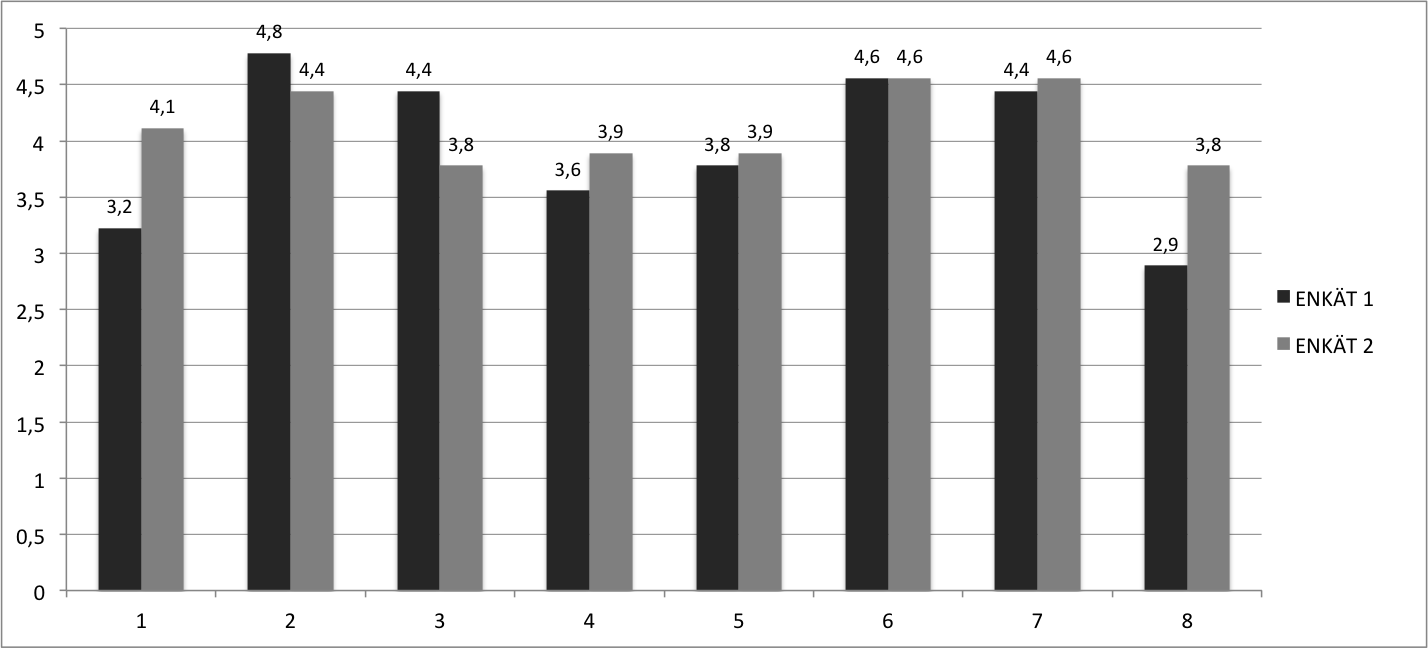
\includegraphics[width=1.0\textwidth]{EnkatResultat.png}\caption{Visar resultaten för den enkät som delats ut vid två tillfällen under kursen (se Appendix B). Första enkäten(mörkgrå) delades ut tre veckor in i projektet och den andra(ljusgrå)sex veckor in}\label{fig:enkat}\end{figure}

Här följer de frågor som fanns med i enkäten som delades ut samt en kort diskussion om resultaten.

\subsubsection{Snabbguiden gjorde det enkelt att förstå grunderna i Git}

Resultatet visar att de tyckte guiden var ok. På första enkäten är detta det näst lägsta resultatet vilket sedn ändrades mycket till den andra enkäten. Vi tror detta mest beror på att de känner sig säkrare med Git och att de inte kommer ihåg den första förvirringen lika väl. Vi är nöjda med resultatet då det var en av de punkter som skulle vara svårast.

\subsubsection{Det är lätt att få igång ett bra workflow (liknande update, update, update, commit för SVN)}

Väldigt högt resultat. Det var det högsta vi fick på första enkäten vilket kan verka en aning märkligt då frågan inte är helt skild från den första. Resultatet gick ner något till den andra enkäten, vilket kan bero på att de börjar använda svårare funktioner. 

\subsubsection{Att använda Terminalen gör att man förstår bättre hur Git fungerar}

Gruppen har även här varit nöjda. Denna fråga har den största sänkningen mellan enkät ett och två. Vi tror att denna sänkningen även här beror på att de använder Git mer avancerat då vissa av dessa funktioner presenterar information man måste ta till sig via terminalen. Vi anser att det är på denna punkt ett grafikt gränssnitt har en stor fördel över terminalen. 

\subsubsection{Git hanterar mergkonflikter på ett bra sätt}

Resultatet speglar ganska bra stämningen i gruppen. Mergekonflikter är alltid tråkigt och vid vissa fall blir folk irriterade på att det borde kunna lösas automatiskt. Samtidigt så får gruppen höra av andra studenter att alternativen inte verkar vara bättre, snarare motsatsen.  

\subsubsection{Git fungerar bra tillsammans med Eclipse}

Förvånandsvärt högt resultat här. Vi valde att inte använda en integrerat pluggin då vi övervägde andra aspekter så som robusthet och förståelse. Vi hade dock förväntat oss ett lägre resultat här efter som man i eclipse själv måste updatera projektet varje gång. Vi tror att det relativt höga resultatet även här kommer för att de har hört av andra studenter att alternativa plugin till SVN har krånglat mycket. 

\subsubsection{När vi stöter på problem med Git kan ni som coacher ofta lösa det}

Folk har bra tilltro till oss som coacher som har bestått genom kursen. Detta visar om något att man inte behöver lång upplärningstid för att lära sig Git då vi coacher var nya till det bara någon månad innan. 

\subsubsection{Mitt helhetsintryck av Git är att det är ett bra versionshanteringssystem}

Ett högt resultat på helhetsintrycket gör att vi är nöjda med valet utav git och rekommenderar det för liknande situationer och framför allt för kursen ifråga. 

\subsubsection{Jag kommer fortsätta använda Git som versionshanteringssystem}

Angående om de skulle använda Git i forstättningen är det lite olika. Ingen har varit med och sett hur man initierar och skapar starten. Vissa har även blivit lite rädda då vi använde oss utav ett eget skrivet shell-script som de ser som mycket svårt. Ökningen till den andra enkät undersökningen tror vi mycket beror på att de känner att de kan hantera svårare funktioner och mer bekväma med de funktioner de redan använder. När de känner att de kan lära sig mer saker inom Git så minskar rädslan för det okända. 

\subsection{Gruppens kommentarer}
I enkäten som gruppen fick fylla fanns även rutor för att fylla i vad de tycker har varit bra och mindre bra med att använda Git. Här följer en summering av deras kommentarer:

\subsubsection{Vad som fungerade bra}
De flesta i gruppen fann det relativt enkelt att förstå grunderna i Git. De tyckte att det kändes stabilt då inga krasher uppkom. Vad som också gillades var att det är svårt att göra destruktiva fel i Git, dvs Git märker om man använder kommandon fel eller i fel ordning och visar varningar. Detta har motverkat små fel som kan ge stora konsekvenser. När det gällde att hantera merge-konflikter i koden fick systemet bra kritik och det var många som kommenterade att det löste många mergar utan att användaren aktivt behövde göra något. Gruppen kände allmänt att de hade fått tillräckligt med stöd från coacherna.

\subsubsection{Vad som kunde fungerat bättre}
Det mest delade svaret på vad som kunde bli bättre var hanteringen av filer som inte ska synkroniseras med repot. Det uppkom en del problem med binära filer som hamnade i repot och ställde till med många små problem. De tyckte även att automatiska merge-konflikter kunde fungerat bättre i textdokument t.ex. JavaDoc där det vid vissa tillfällen uppkom, vad gruppen tyckte var, onödiga merge-konflikter. Till sist var det ett antal i gruppen som önskade att det hade funnits ett grafiskt användargränssnitt i form av ett plugin till Eclipse. 

\subsubsection{Coachernas reflektioner}
Efter att ha läst igenom och sammanställt gruppens individuella kommentarer kommer vi till slutsatsen att vi är nöjda med studien. Det var övervägande positiv kritik från gruppen och det mesta av de problem som beskrevs kan på ett eller annat sätt åtgärdas.

Önskemålet om ett grafiskt användargränssnitt kan enkelt uppfyllas med pluginet EGit till Eclipse. Anledningen till att detta inte användes var att det inte kunde installeras på ett enkelt sätt på skolans datorer. I den senaste versionen av Eclipse är detta plugin dessutom inbyggt och integrerat med användargränssnittet.

Problemet med att filer som inte skulle ligga på repot hamnade där ändå kan vi som coacher ta på oss. I Git definierar man en fil med olika mappar, filtyper och filnamn som ska exkluderas från repot. När vi skrev ihop den filen misstolkade vi hur mappar skulle definieras. Efter att problemet uppdagats och felet åtgärdats fungerade allt bra.